% =====================================================================
%  Defense deck - Generative Modelling of Maritime AIS Trajectories
%  Beamer, styled after the École Polytechnique bachelor-thesis report
%  (report/report_v3.tex): Times serif body, EP red + navy palette.
%  Build:  pdflatex defense_presentation.tex   (run twice)
% =====================================================================
\documentclass[aspectratio=169,11pt]{beamer}

% ---- fonts: match the report (times / mathptmx serif) ---------------
\usepackage[T1]{fontenc}
\usepackage{mathptmx}            % Times, same as report's \usepackage{times}
\renewcommand{\familydefault}{\rmdefault}
\usefonttheme{serif}

\usepackage{graphicx}
\usepackage{booktabs}
\usepackage{xcolor}
\usepackage{colortbl}
\usepackage{tikz}
\usetikzlibrary{arrows.meta,positioning,calc}

\graphicspath{{figures/}{report/figures/}{report/}}

% ---- palette (mirrors the report) -----------------------------------
\definecolor{epnavy}{HTML}{1B2A4A}
\definecolor{epred}{HTML}{C1002A}
\definecolor{epgrey}{HTML}{5A5A5A}
\definecolor{eplight}{HTML}{E9ECF2}

% ---- clean academic theme ------------------------------------------
\usetheme{default}
\usecolortheme{default}
\setbeamercolor{normal text}{fg=black}
\setbeamercolor{structure}{fg=epnavy}
\setbeamercolor{frametitle}{fg=epnavy}
\setbeamercolor{title}{fg=epnavy}
\setbeamercolor{itemize item}{fg=epred}
\setbeamercolor{itemize subitem}{fg=epred}
\setbeamerfont{frametitle}{series=\bfseries,size=\Large}
\setbeamertemplate{navigation symbols}{}
\setbeamertemplate{itemize item}{\small\raise0.4pt\hbox{\textcolor{epred}{\rule{5pt}{5pt}}}}
\setbeamertemplate{itemize subitem}{\textcolor{epred}{--}}

% blocks styled in the EP palette
\setbeamertemplate{blocks}[rounded][shadow=false]
\setbeamercolor{block title}{bg=epnavy,fg=white}
\setbeamercolor{block body}{bg=eplight,fg=black}

% frame title with a thin EP-red rule underneath
\setbeamertemplate{frametitle}{%
  \vskip0.5em%
  \begin{beamercolorbox}[wd=\paperwidth,leftskip=0.6cm,rightskip=0.6cm]{frametitle}%
    {\bfseries\Large\insertframetitle}%
    \ifx\insertframesubtitle\empty\else
      \\[0.15em]{\normalfont\itshape\small\color{epgrey}\insertframesubtitle}%
    \fi
    \par\vskip2pt%
    {\color{epred}\rule{2.6cm}{1.6pt}}%
  \end{beamercolorbox}%
}

% footer: discreet slide number only
\setbeamertemplate{footline}{%
  \hbox{\begin{beamercolorbox}[wd=\paperwidth,ht=2.2ex,dp=1.2ex,leftskip=0.6cm,rightskip=0.6cm]{}%
    {\scriptsize\color{epgrey}\hfill\insertframenumber}%
  \end{beamercolorbox}}%
}

% caption helper
\newcommand{\fcap}[1]{\par\vskip2pt{\footnotesize\itshape\color{epgrey}#1}}
\newcommand{\lead}[1]{\textcolor{epnavy}{\bfseries #1}}

\title{Generative Modelling of Maritime AIS Trajectories}
\author{Andrei-Valentin \c{S}tirbu}
\date{}

% =====================================================================
\begin{document}
% =====================================================================

% ---- Title slide ----------------------------------------------------
{\setbeamertemplate{footline}{}
\begin{frame}[plain]
  \begin{tikzpicture}[remember picture,overlay]
    \fill[epred] (current page.north west) rectangle ([yshift=-0.18cm]current page.north east);
  \end{tikzpicture}
  \vspace{0.2em}
  \begin{center}
    
\includegraphics[height=1.7cm]{logo-EP-vertical}\\[1.0em]
    {\LARGE\bfseries\color{epnavy} Generative Modelling of Maritime AIS Trajectories}\\[0.35em]
    {\LARGE\bfseries\color{epnavy} with Retrieval-Augmented Transformers}\\[0.7em]
    {\large\itshape\color{epgrey} A Land-Aware, Water-Strict Route Generator\\[0.15em]
     from Start, End and Vessel Type}\\[0.8em]
    {\color{epred}\rule{3cm}{1.4pt}}\\[0.9em]
    {\normalsize
     \lead{Author:}\ \ Andrei-Valentin \c{S}tirbu - \'Ecole Polytechnique\\[0.35em]
     \lead{Advisor:}\ \ Davide Buscaldi - LIX, \'Ecole Polytechnique \& Sorbonne Universit\'e\\[0.5em]
     {\itshape\color{epgrey} Lab Research Project}}
  \end{center}
\end{frame}}

% ---- 2. Motivation --------------------------------------------------
\begin{frame}{Why learn maritime routes?}{AIS broadcasts every large vessel's position - $\sim$$10^8$ pings per year (NOAA, 2024)}
  \begin{columns}[T]
    \column{0.5\textwidth}
      \begin{itemize}\setlength\itemsep{0.7em}
        \item \lead{Question:} given only (start, end, vessel type), can we sketch a plausible route?
        \item \lead{Data:} 2024 US corpus $\approx 9.9\times10^7$ rows, ${\sim}6\times10^5$ segments
        \item \lead{Value:} traffic simulation, storm-risk routing, ETA, anomaly detection
      \end{itemize}
    \column{0.5\textwidth}
      \centering
      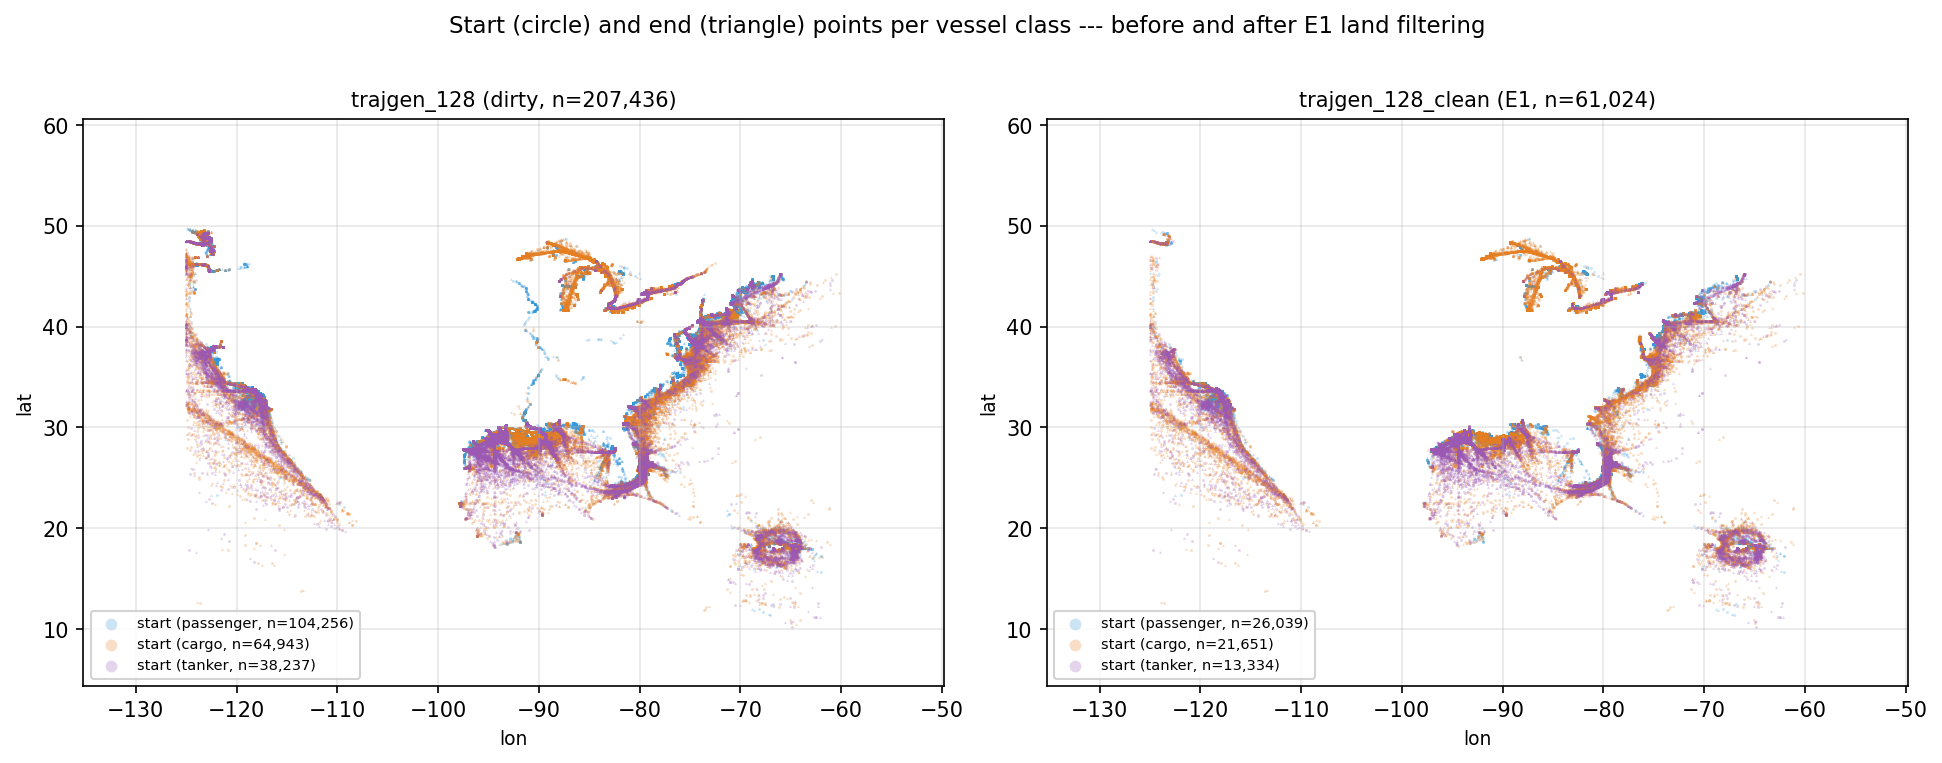
\includegraphics[width=\linewidth]{data_start_end}
      \fcap{Start (green) and end (red) distributions across the US coastal corpus}
  \end{columns}
\end{frame}

% ---- 3. Problem statement ------------------------------------------
\begin{frame}{Problem: constrained full-route generation}{Generate $T=128$ waypoints minimising ADE under two constraints}
  \begin{columns}[T]
    \column{0.56\textwidth}
      \begin{itemize}\setlength\itemsep{0.6em}
        \item \lead{Input $\to$ output:} $q=(p_1,p_T,v)\ \to\ \hat\tau=(\hat p_1,\dots,\hat p_{128})$
        \item \lead{Objective:} minimise $\mathrm{ADE}=\frac1T\sum_t \mathrm{haversine}(\hat p_t,p_t)$
        \item \lead{C1 - endpoint-exact:} $\hat p_1=p_1,\ \hat p_T=p_T$
        \item \lead{C2 - water-valid:} $\mathrm{sdf}(\hat p_t)\le\theta$ for all $t$
      \end{itemize}
      \vskip0.6em
      {\small\color{epred} The three objectives pull against each other; baseline = great-circle geodesic.}
    \column{0.44\textwidth}
      \centering
      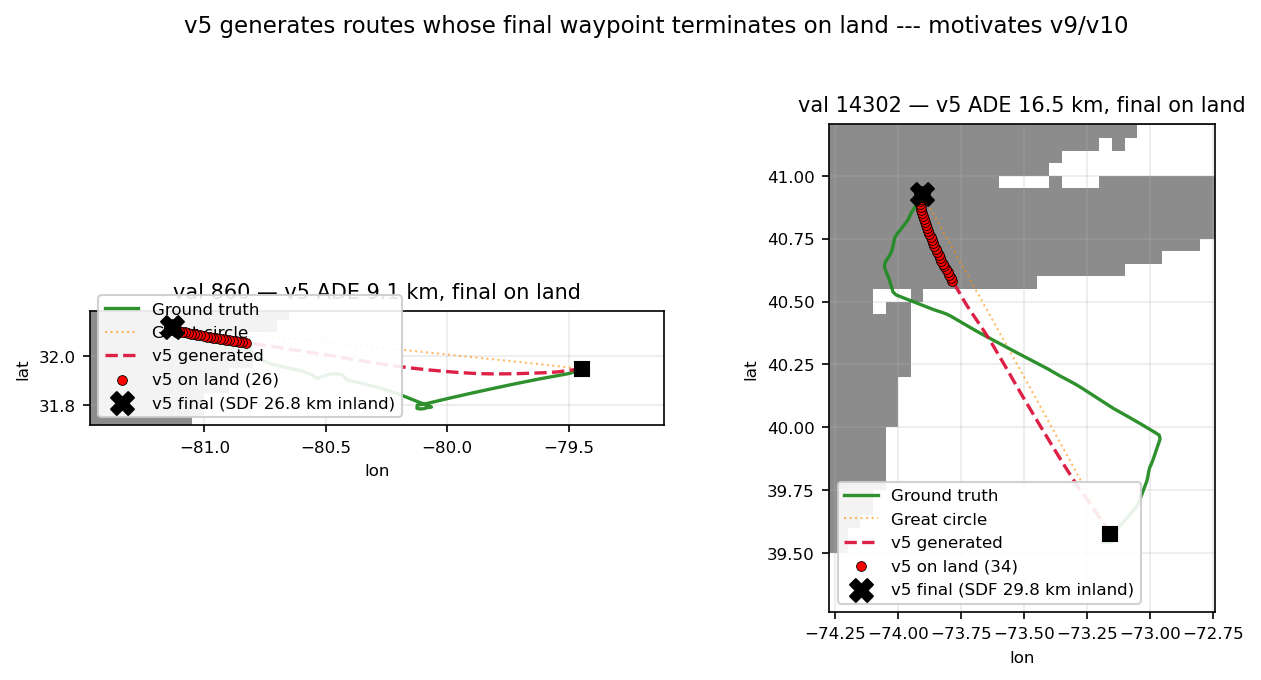
\includegraphics[width=\linewidth]{motiv_v5_lands_on_coast}
      \fcap{A model that ignores C2 runs aground on the coast}
  \end{columns}
\end{frame}

% ---- 4. Why it's hard ----------------------------------------------
\begin{frame}{Four reasons it is hard}
  \begin{itemize}\setlength\itemsep{0.35em}
    \item \lead{Irregular constraint surface:} land/water flips over a few km; narrow inlets need $0.005^\circ$
    \item \lead{Multimodal routes:} many valid paths per query - ADE penalises the ``wrong'' valid mode
    \item \lead{Two orders of magnitude:} 20\,km hops \dots\ 2000\,km voyages - no single bias fits both
    \item \lead{Noisy ground truth:} even cleaned GT crosses land $10.83\%$ @10\,km before filtering
  \end{itemize}
  \vskip0.4em
  \begin{columns}[T]
    \column{0.5\textwidth}\centering
      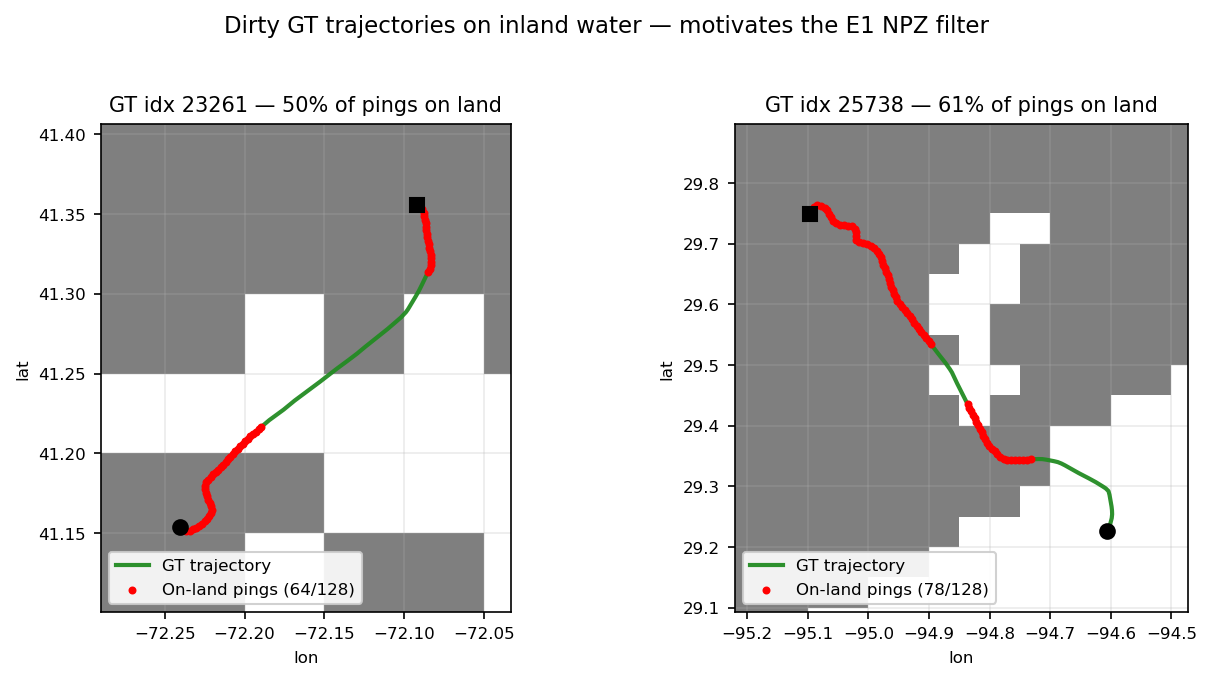
\includegraphics[height=3.3cm]{motiv_dirty_gt_on_river}
      \fcap{Dirty GT track running up a river}
    \column{0.5\textwidth}\centering
      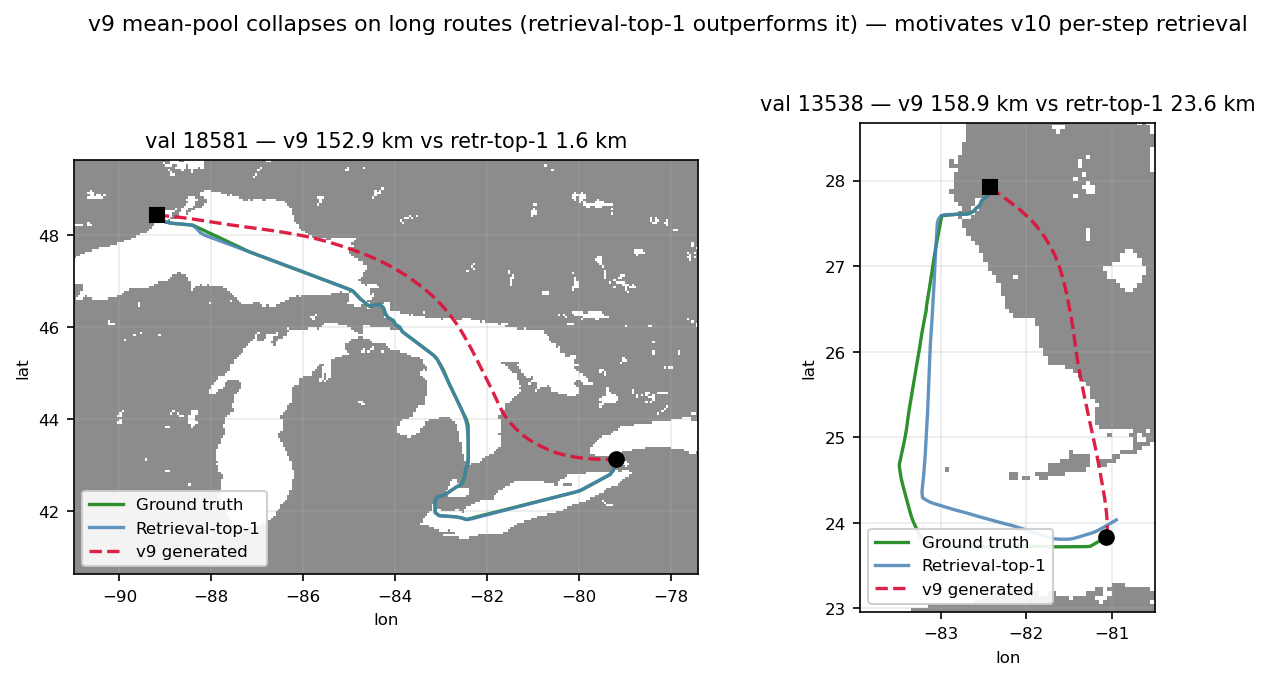
\includegraphics[height=3.3cm]{motiv_v9_long_route_collapse}
      \fcap{Mean-pool retrieval (v9) collapses on a long route}
  \end{columns}
\end{frame}

% ---- 5. Data pipeline ----------------------------------------------
\begin{frame}{End-to-end production pipeline}{Raw NOAA archives $\to$ cleaned 128-waypoint corpus $\to$ trained model $\to$ post-processed route}
  \begin{columns}[c]
    \column{0.66\textwidth}\centering
      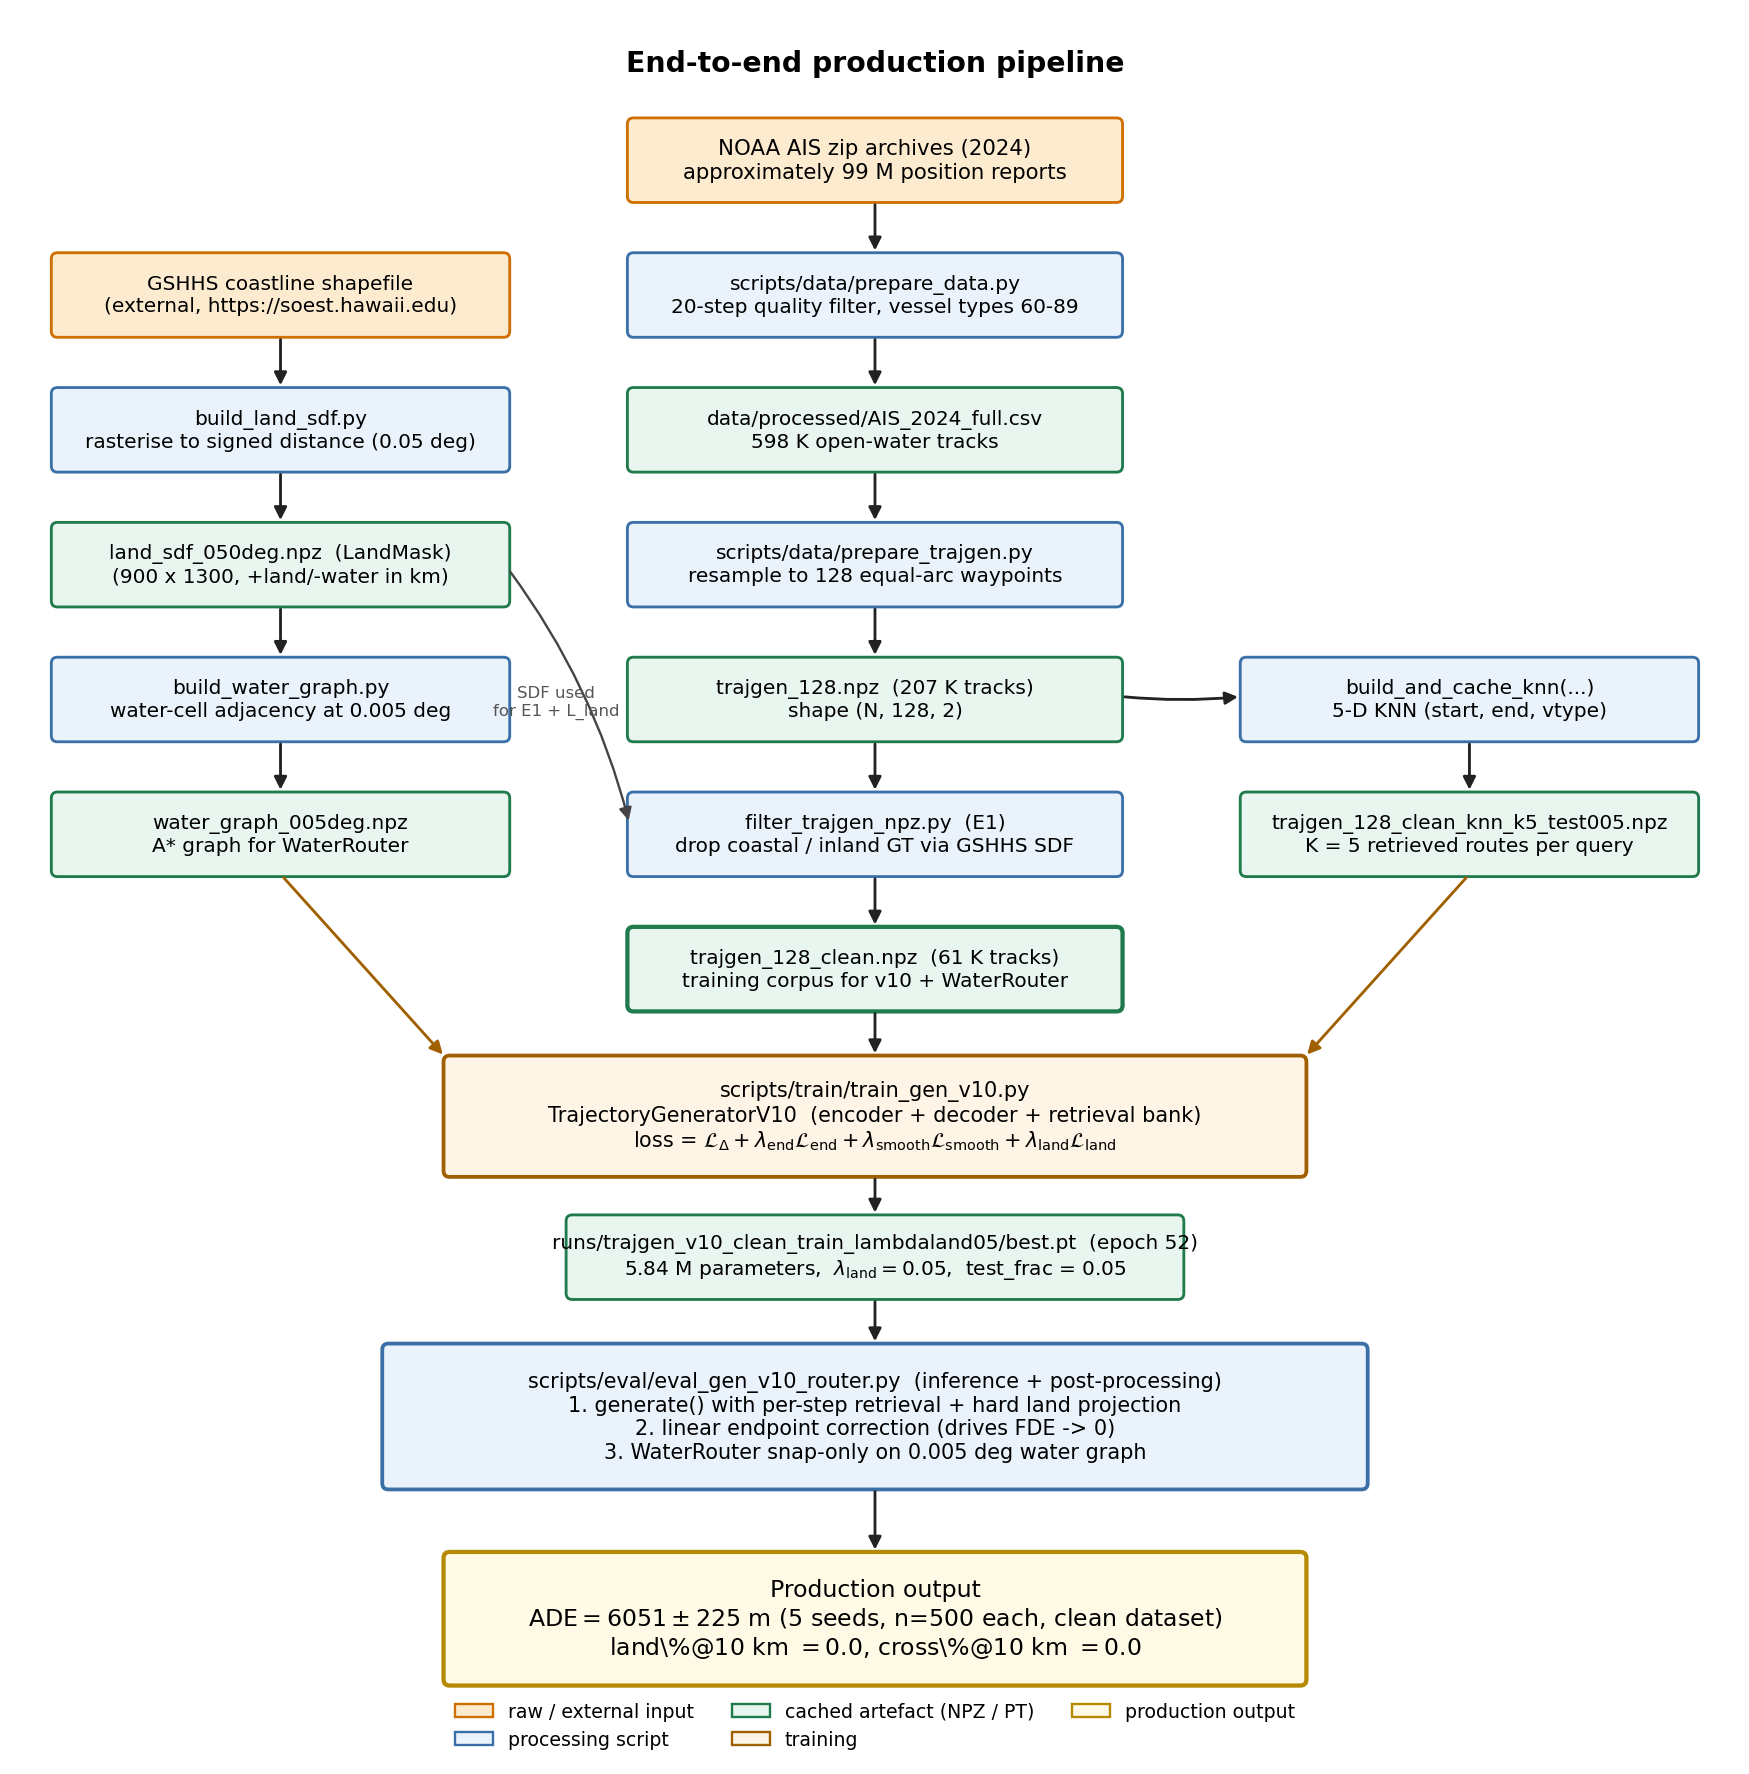
\includegraphics[height=5.4cm]{data_pipeline}
    \column{0.34\textwidth}
      \begin{itemize}\setlength\itemsep{0.55em}
        \item \lead{Orange:} raw / external input
        \item \lead{Blue:} processing scripts
        \item \lead{Green:} cached artefacts (built once)
        \item \lead{Yellow:} training
        \item \lead{Gold:} production output
      \end{itemize}
  \end{columns}
\end{frame}

% ---- 6. Data cleaning (E1) -----------------------------------------
\begin{frame}{Data quality: the single largest intervention}{E1 land filter on the GSHHS shoreline $\to$ leak-free clean corpus}
  \begin{itemize}\setlength\itemsep{0.3em}
    \item \lead{Problem:} unfiltered 128-pt GT crosses land $10.83\%$ @10\,km
    \item \lead{Filter:} drop tracks with $>$2\% land fraction or $>$10\,km penetration $\Rightarrow$ 61k/207k kept
    \item \lead{Impact:} larger than any single architecture change
  \end{itemize}
  \vskip0.3em
  \begin{columns}[T]
    \column{0.5\textwidth}\centering
      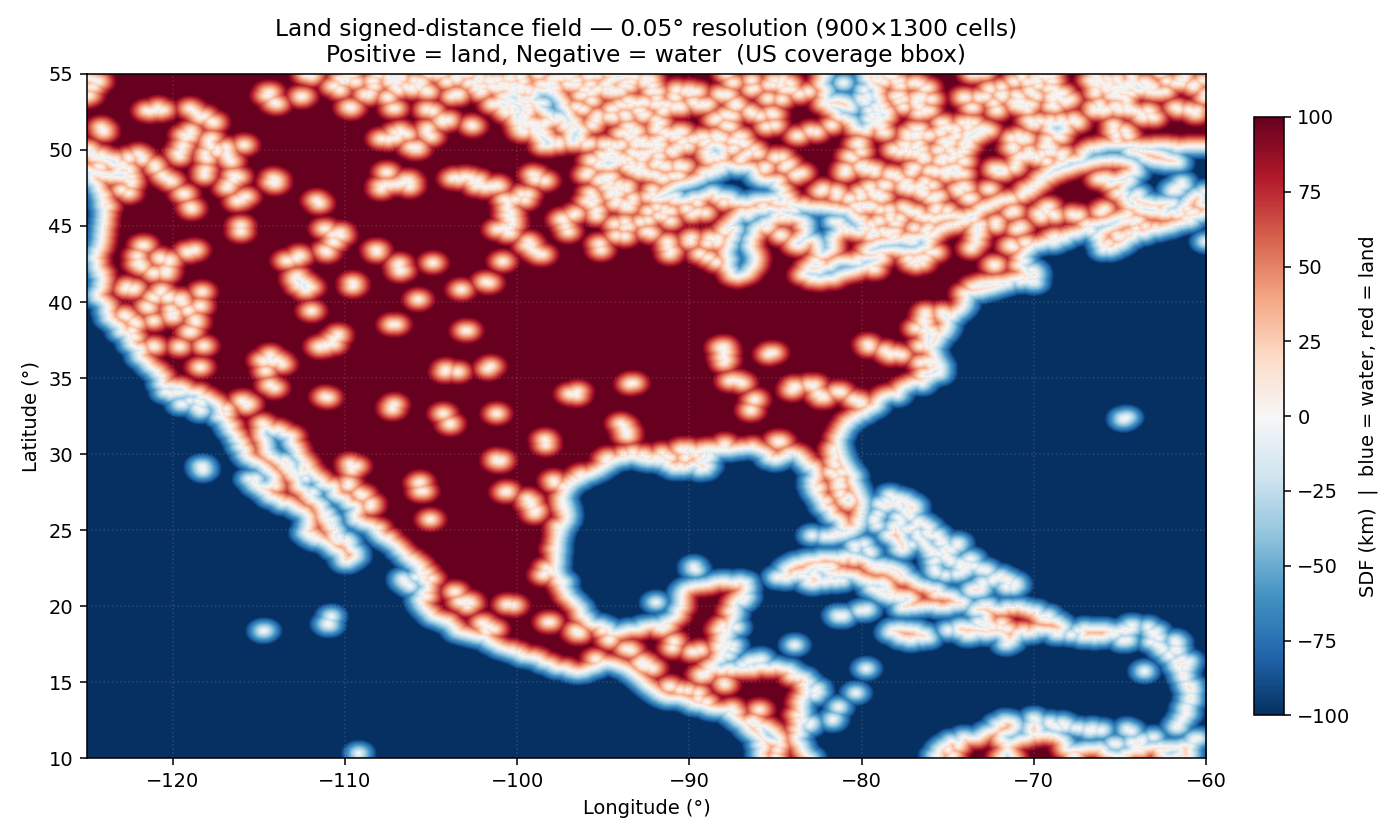
\includegraphics[width=\linewidth,height=3.1cm,keepaspectratio]{land_sdf}
      \fcap{Signed-distance field: $+$ = land, $-$ = water}
    \column{0.5\textwidth}\centering
      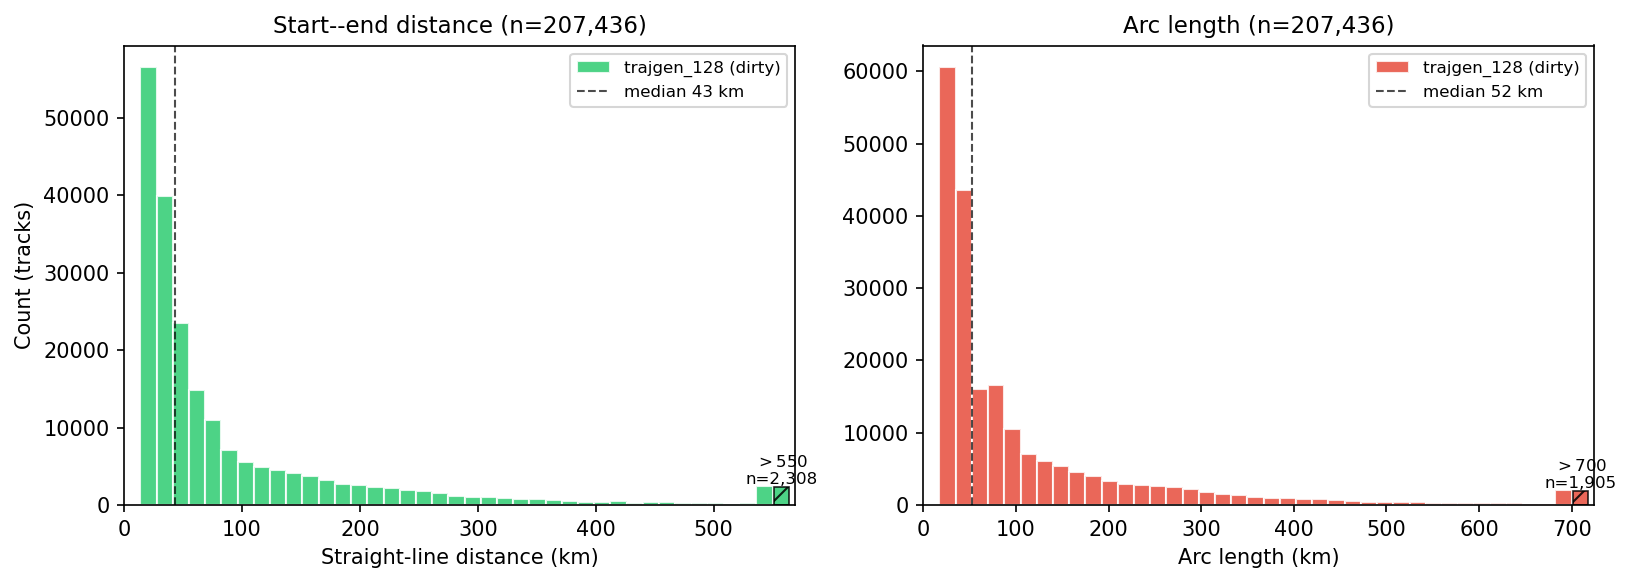
\includegraphics[width=\linewidth,height=3.1cm,keepaspectratio]{data_distributions}
      \fcap{Corpus distributions after cleaning}
  \end{columns}
\end{frame}

% ---- 7. Architecture -----------------------------------------------
\begin{frame}{Model architecture (v10)}{Retrieval-augmented encoder--decoder - the production model}
  \begin{columns}[c]
    \column{0.60\textwidth}
      \hspace*{-0.5cm}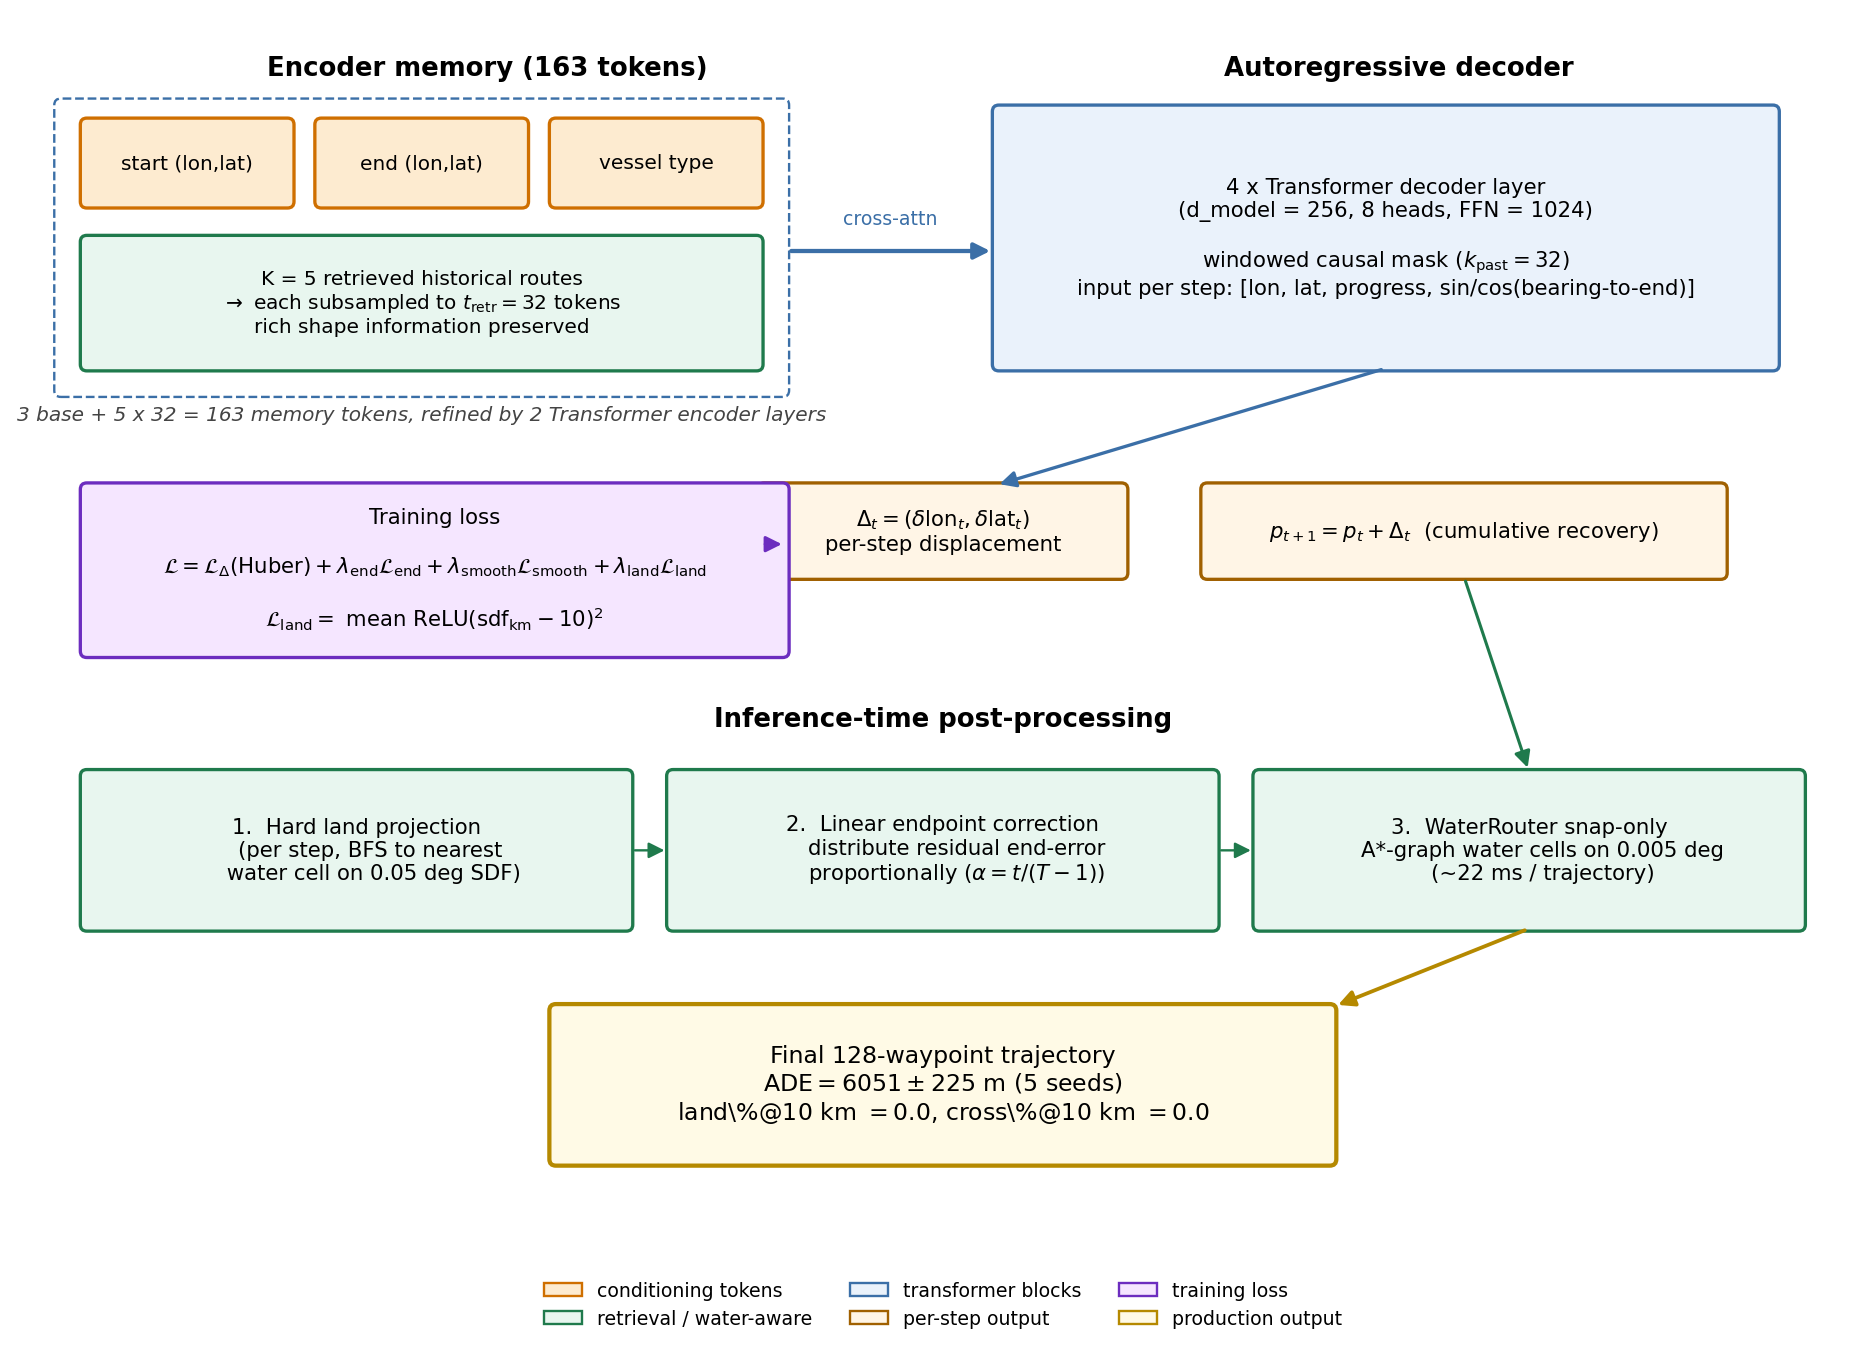
\includegraphics[width=1.05\linewidth,height=5.3cm,keepaspectratio]{architecture_v10}
    \column{0.40\textwidth}
      \begin{itemize}\setlength\itemsep{0.6em}
        \item \lead{163 memory tokens:} 3 conditioning $+\ 5\times32$ retrieval
        \item \lead{Windowed-causal decoder:} one displacement/step, $k_{\text{past}}=32$
        \item \lead{Four-term loss:} Huber $+$ endpoint $+$ smoothness $+$ land
        \item \lead{Three inference passes:} project $\to$ endpoint fix $\to$ snap
      \end{itemize}
  \end{columns}
\end{frame}

% ---- 8. Idea 1: retrieval ------------------------------------------
\begin{frame}{Key idea 1 - per-step retrieval}{The largest single architectural lever: $>$25\% ADE reduction}
  \begin{itemize}\setlength\itemsep{0.3em}
    \item \lead{How:} $K=5$ historical neighbours $\times\ t_{\text{retr}}=32$ steps as memory tokens
    \item \lead{Why it beats v9:} decoder cross-attends \emph{per step} - no mean-pool shape collapse
    \item \lead{Evidence:} ADE correlates with top-1 neighbour distance ($\rho=+0.40$, short bucket)
    \item \lead{Lesson:} try non-parametric memory before scaling the parametric model
  \end{itemize}
  \vskip0.2em
  \centering
  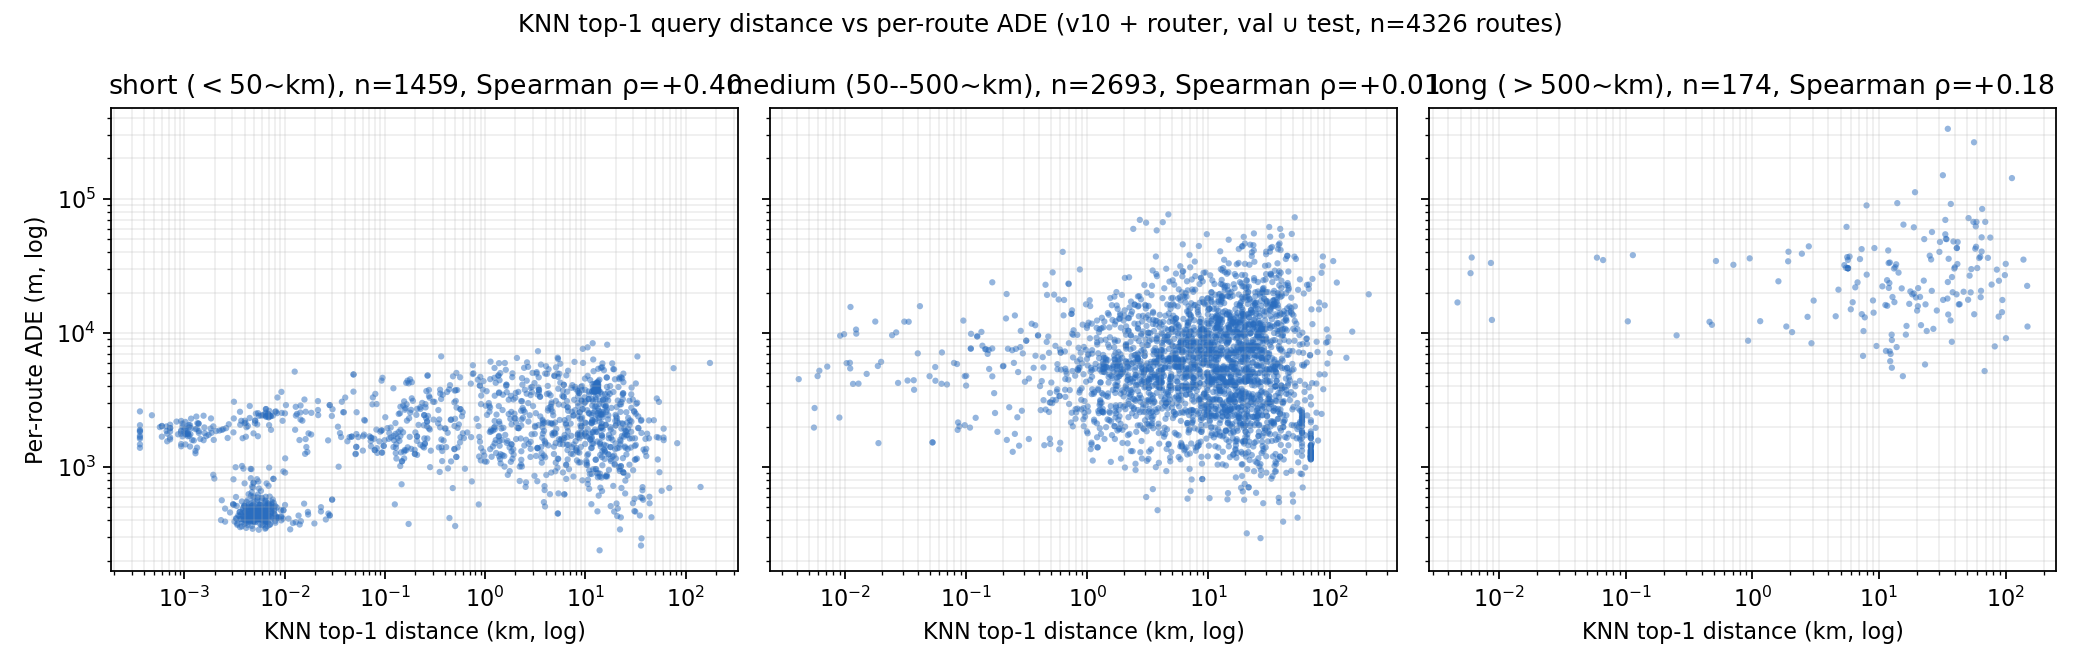
\includegraphics[width=0.95\linewidth,height=3.0cm,keepaspectratio]{retrieval_quality_scatter}
  \fcap{Per-route ADE vs nearest-neighbour distance - retrieval is doing real work}
\end{frame}

% ---- 9. Idea 2: land loss + snap -----------------------------------
\begin{frame}{Key idea 2 - land-aware loss \& WaterRouter snap}{Differentiable SDF penalty in training; snap-to-water at inference $\to$ 0\% crossings}
  \begin{itemize}\setlength\itemsep{0.25em}
    \item \lead{Training:} $L_{\text{land}}=\mathrm{mean}\,\mathrm{ReLU}(\mathrm{sdf}-\theta)^2$ via bilinear \texttt{grid\_sample}
    \item \lead{Inference:} snap any violating waypoint to nearest \emph{connected} water cell ($0.005^\circ$ graph)
    \item \lead{Cost:} ${\sim}22$\,ms/route, no ADE penalty on the clean corpus
  \end{itemize}
  \vskip0.3em
  \begin{columns}[T]
    \column{0.46\textwidth}\centering
      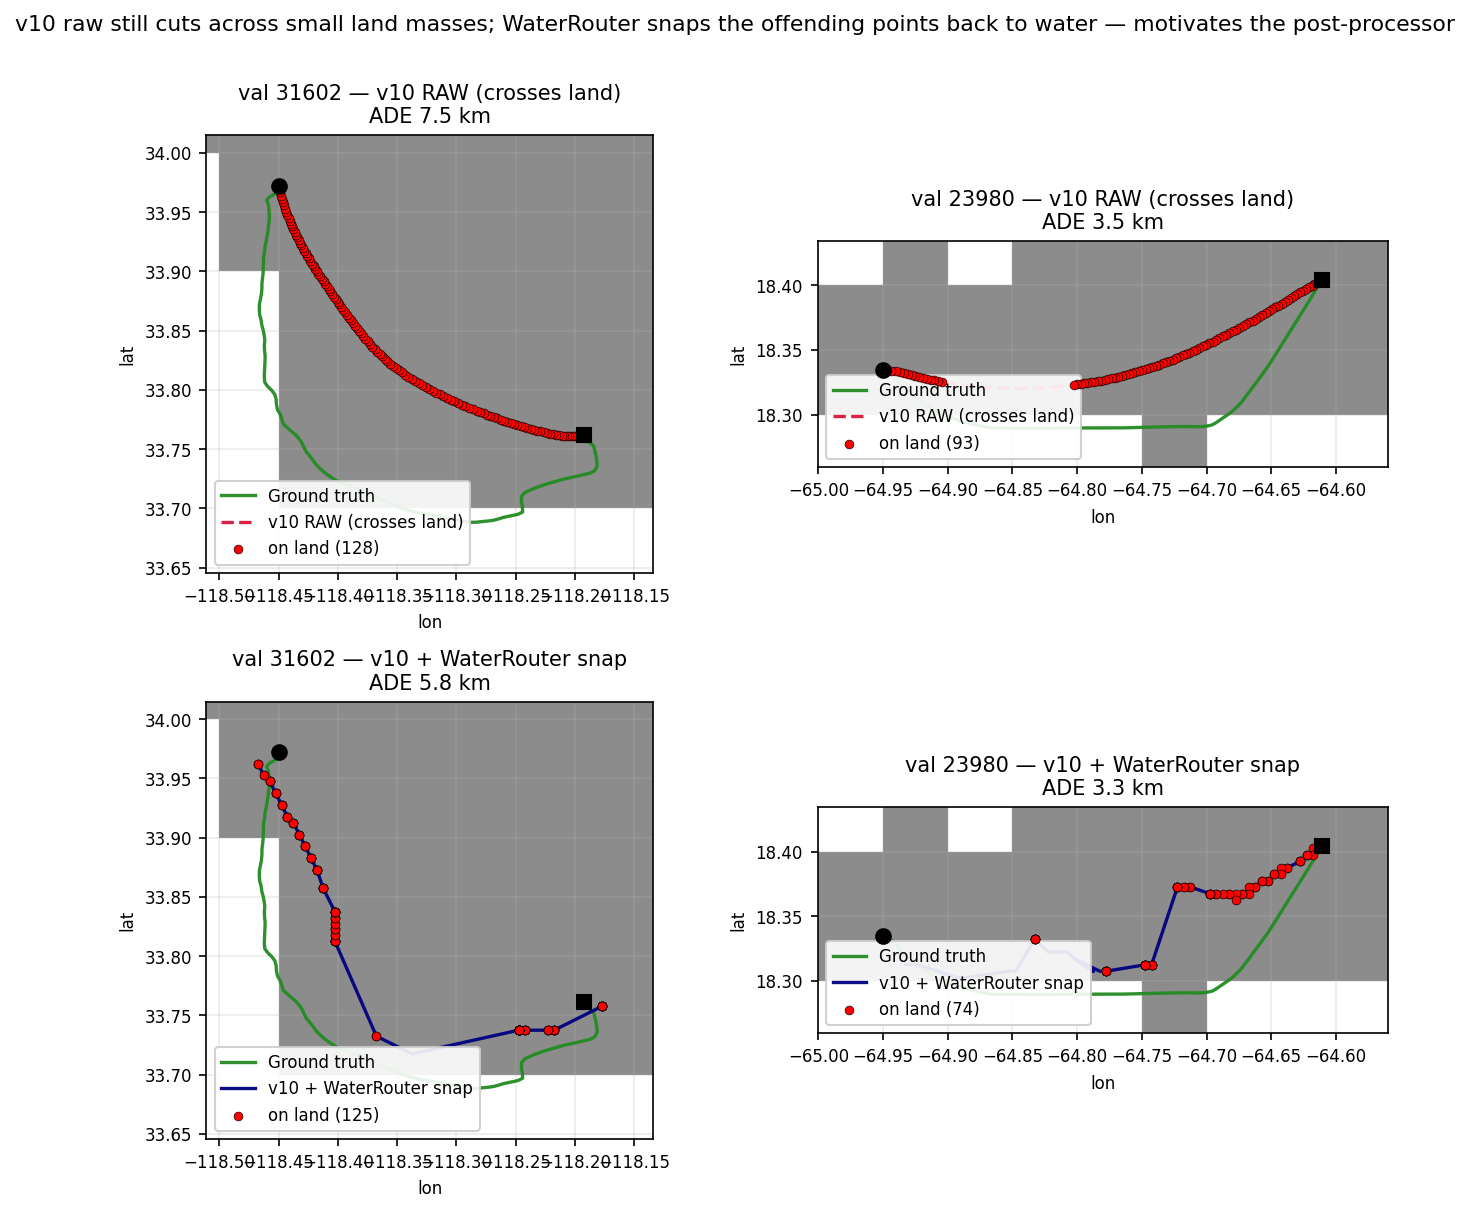
\includegraphics[height=3.1cm]{motiv_v10_raw_crosses_land}
      \fcap{Raw v10 output still clips a headland \dots}
    \column{0.54\textwidth}\centering
      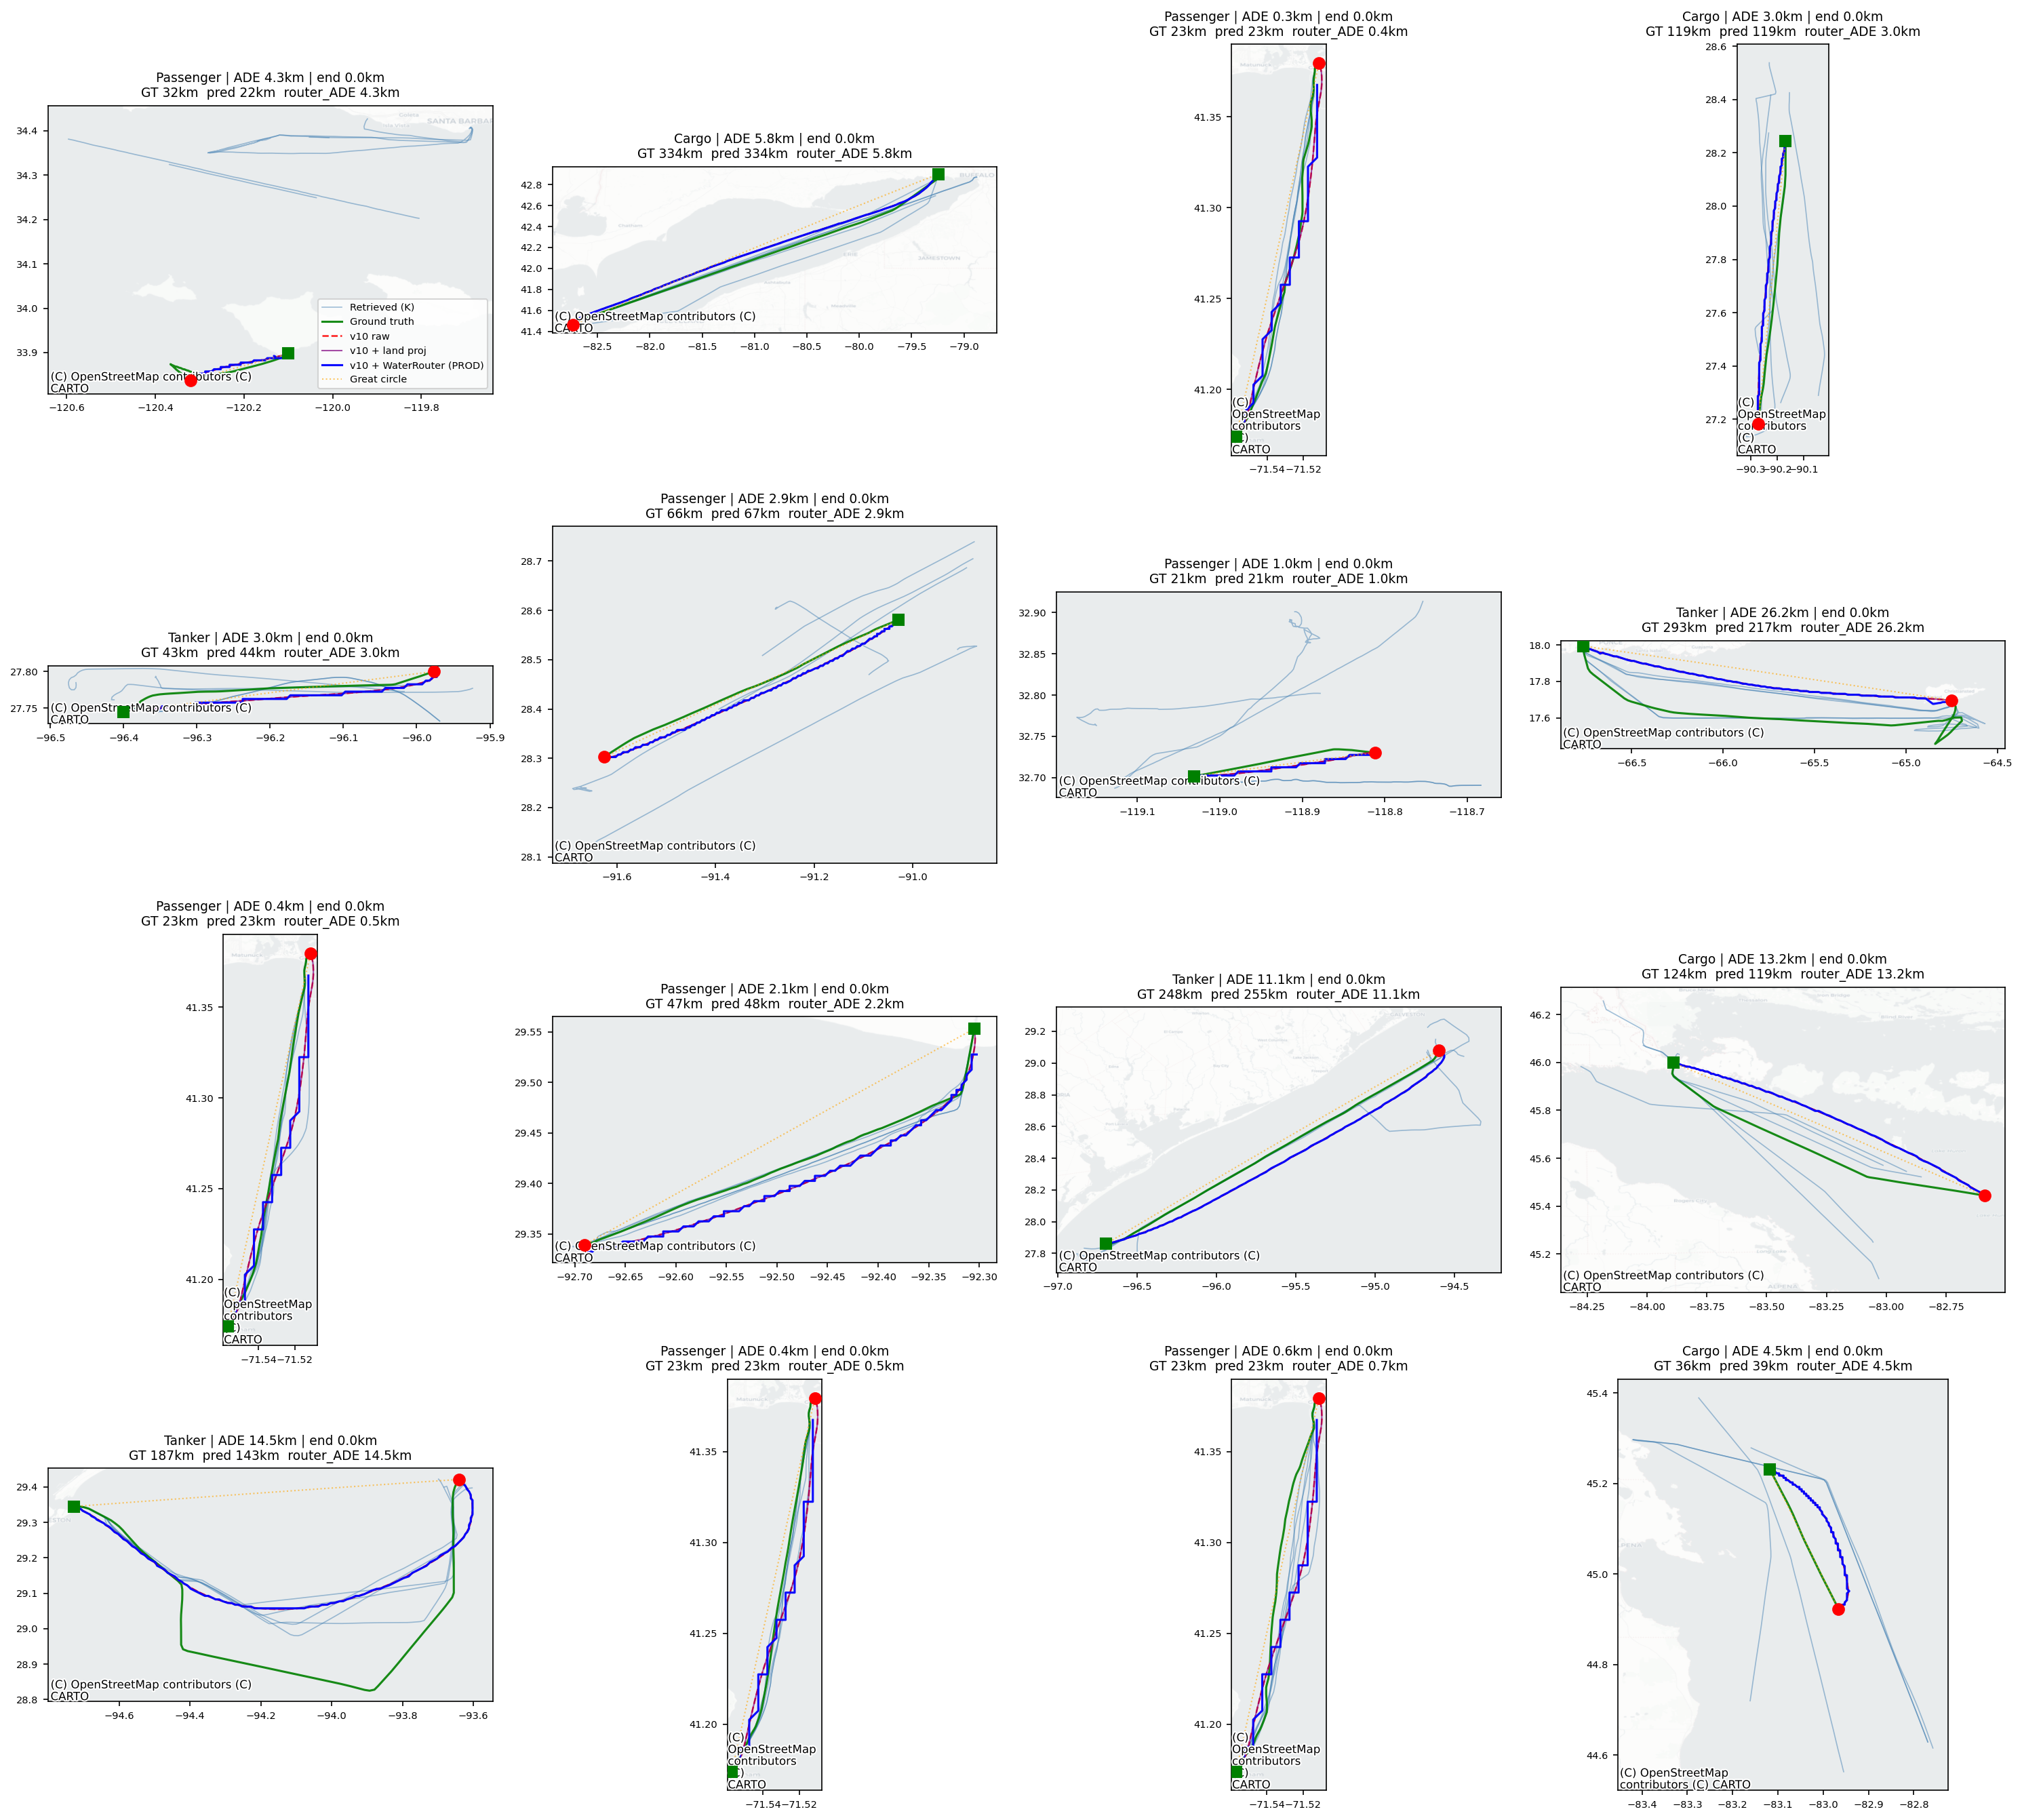
\includegraphics[height=3.1cm]{viz_v10_clean}
      \fcap{\dots\ WaterRouter snaps it back onto water}
  \end{columns}
\end{frame}

% ---- 10. Inference pipeline (tikz) ---------------------------------
\begin{frame}{Inference: three post-processing passes}
  \vskip0.6em
  \centering
  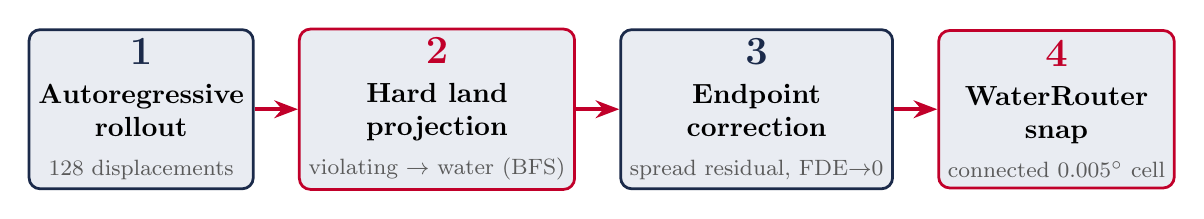
\begin{tikzpicture}[
      node distance=0.55cm,
      box/.style={rounded corners,draw,line width=1pt,minimum width=2.7cm,
                  minimum height=2.0cm,align=center,fill=eplight},
      arr/.style={-{Stealth[length=3mm]},line width=1.4pt,epred}]
    \node[box,draw=epnavy] (a) {{\Large\bfseries\color{epnavy}1}\\[2pt]
      \textbf{Autoregressive}\\\textbf{rollout}\\[2pt]{\footnotesize\color{epgrey}128 displacements}};
    \node[box,draw=epred,right=of a] (b) {{\Large\bfseries\color{epred}2}\\[2pt]
      \textbf{Hard land}\\\textbf{projection}\\[2pt]{\footnotesize\color{epgrey}violating $\to$ water (BFS)}};
    \node[box,draw=epnavy,right=of b] (c) {{\Large\bfseries\color{epnavy}3}\\[2pt]
      \textbf{Endpoint}\\\textbf{correction}\\[2pt]{\footnotesize\color{epgrey}spread residual, FDE$\to$0}};
    \node[box,draw=epred,right=of c] (d) {{\Large\bfseries\color{epred}4}\\[2pt]
      \textbf{WaterRouter}\\\textbf{snap}\\[2pt]{\footnotesize\color{epgrey}connected $0.005^\circ$ cell}};
    \draw[arr] (a) -- (b); \draw[arr] (b) -- (c); \draw[arr] (c) -- (d);
  \end{tikzpicture}
  \vskip1.4em
  {\itshape All four passes are post-hoc - no retraining - and together satisfy C1 (endpoint) and C2 (water-strict).}
\end{frame}

% ---- 11. Headline results ------------------------------------------
\begin{frame}{Headline results}{v10 + router: $-32\%$ ADE vs great-circle, 0.0\% land crossings}
  \begin{columns}[T]
    \column{0.62\textwidth}
      \vskip0.3em
      {\small
      \setlength\tabcolsep{4pt}
      \begin{tabular}{lrrc}
        \toprule
        \textbf{Method} & ADE (m) & FDE (m) & \shortstack{cross\%\\@10\,km} \\
        \midrule
        \rowcolor{eplight}\textbf{v10 + router (prod.)} & $\mathbf{5930{\pm}372}$ & $608$ & $0.04$ \\
        v10 raw (same ckpt)        & $5913{\pm}384$  & $0$     & $1.88$ \\
        Great-circle + snap        & $8484{\pm}597$  & $581$   & $0.20$ \\
        Great-circle baseline      & $8735{\pm}651$  & $0$     & $8.80$ \\
        Retrieval top-1 (0-train)  & $11667{\pm}636$ & $11832$ & $0.00$ \\
        \bottomrule
      \end{tabular}}
      \vskip0.6em
      \centering
      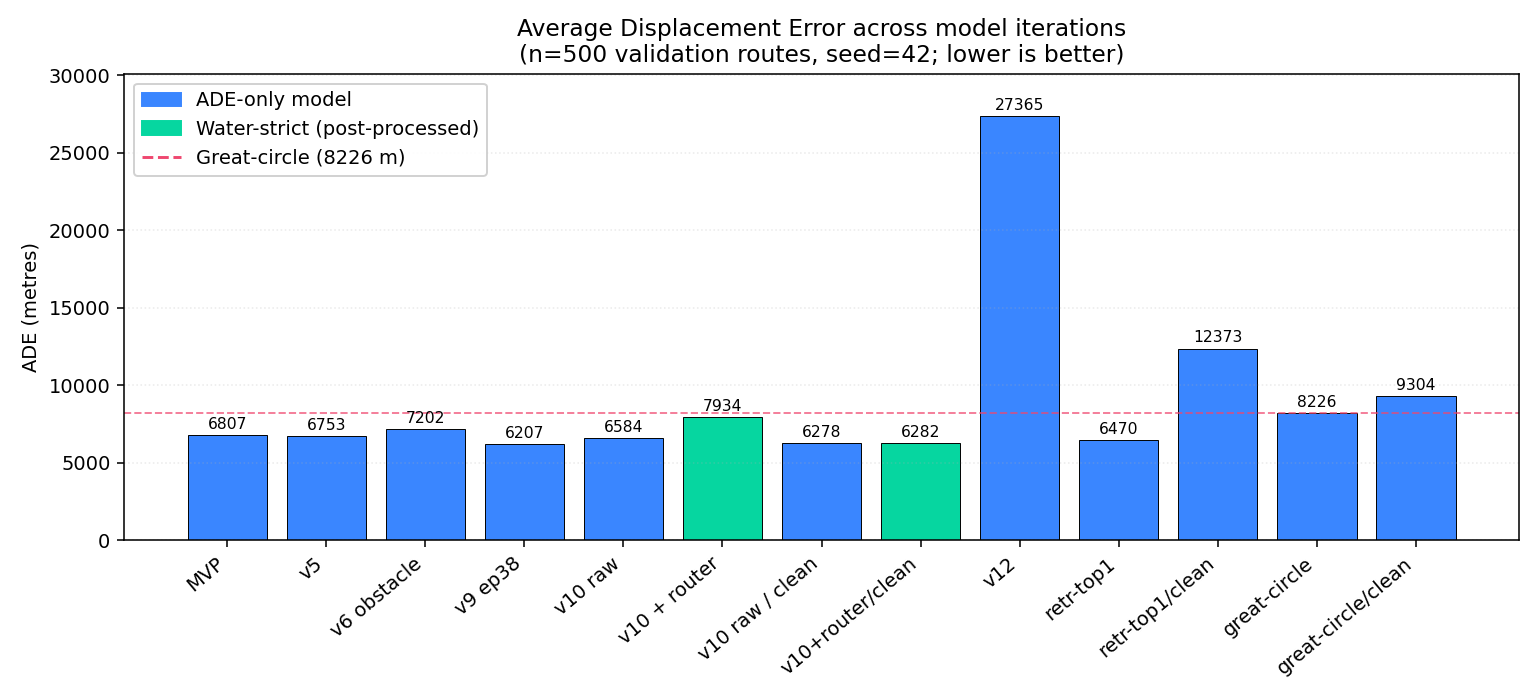
\includegraphics[width=0.92\linewidth,height=3.0cm,keepaspectratio]{ade_by_model}
      \fcap{ADE by method}
    \column{0.38\textwidth}
      \vskip0.8em
      {\small
      \lead{Setup:} 5-seed mean $\pm$ std, disjoint 500-route subsamples\\[0.8em]
      \lead{Best ADE:} $-32\%$ vs great-circle\\[0.8em]
      \lead{Water-strict:} only learned method at 0\% crossings\\[0.8em]
      \lead{Free validity:} router costs $+17$\,m ADE vs raw}
  \end{columns}
\end{frame}

% ---- 12. Length-bucketed + qualitative -----------------------------
\begin{frame}{Where the model wins - and qualitative routes}{Largest gains on medium/long voyages; great-circle still best on very short hops}
  \begin{columns}[c]
    \column{0.5\textwidth}\centering
      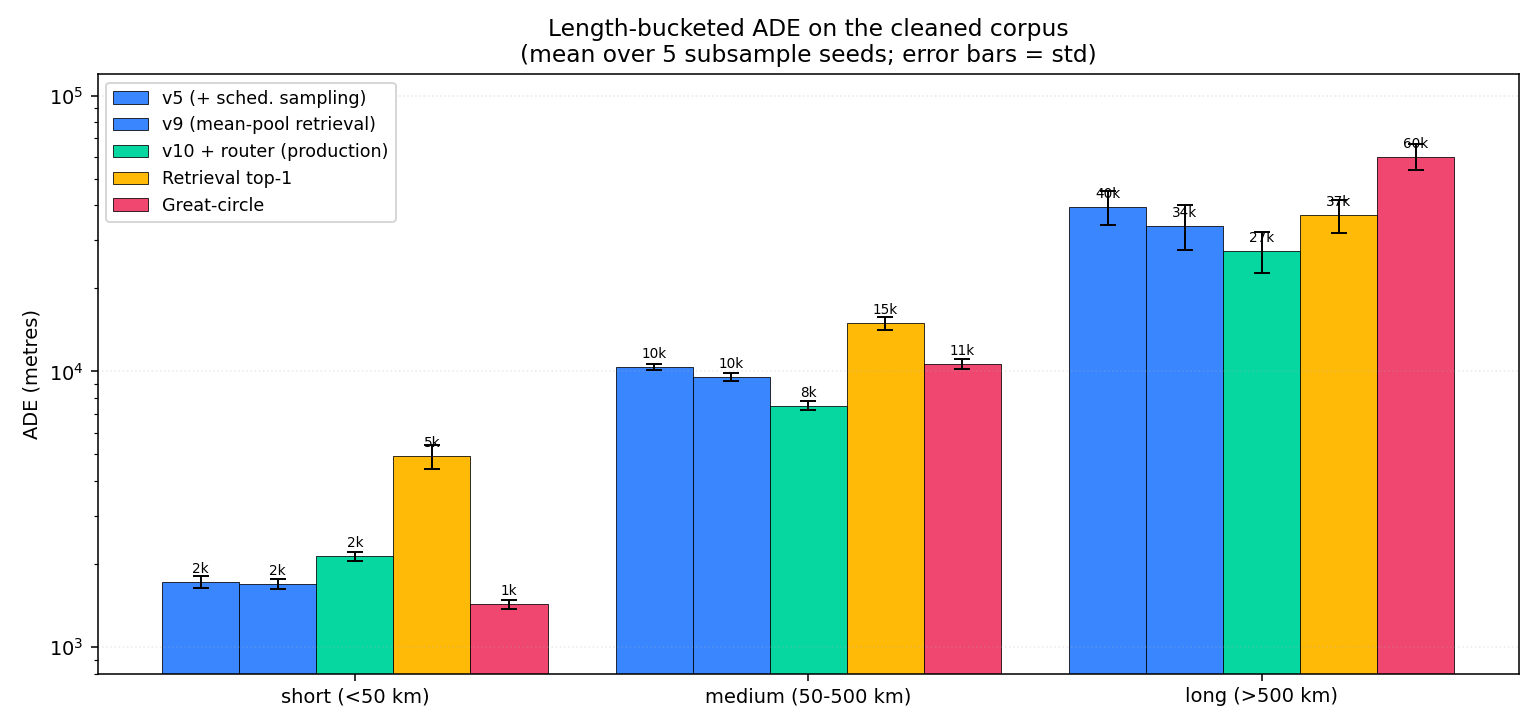
\includegraphics[width=\linewidth]{length_bucketed_ade}
      \fcap{ADE by route-length bucket}
    \column{0.5\textwidth}\centering
      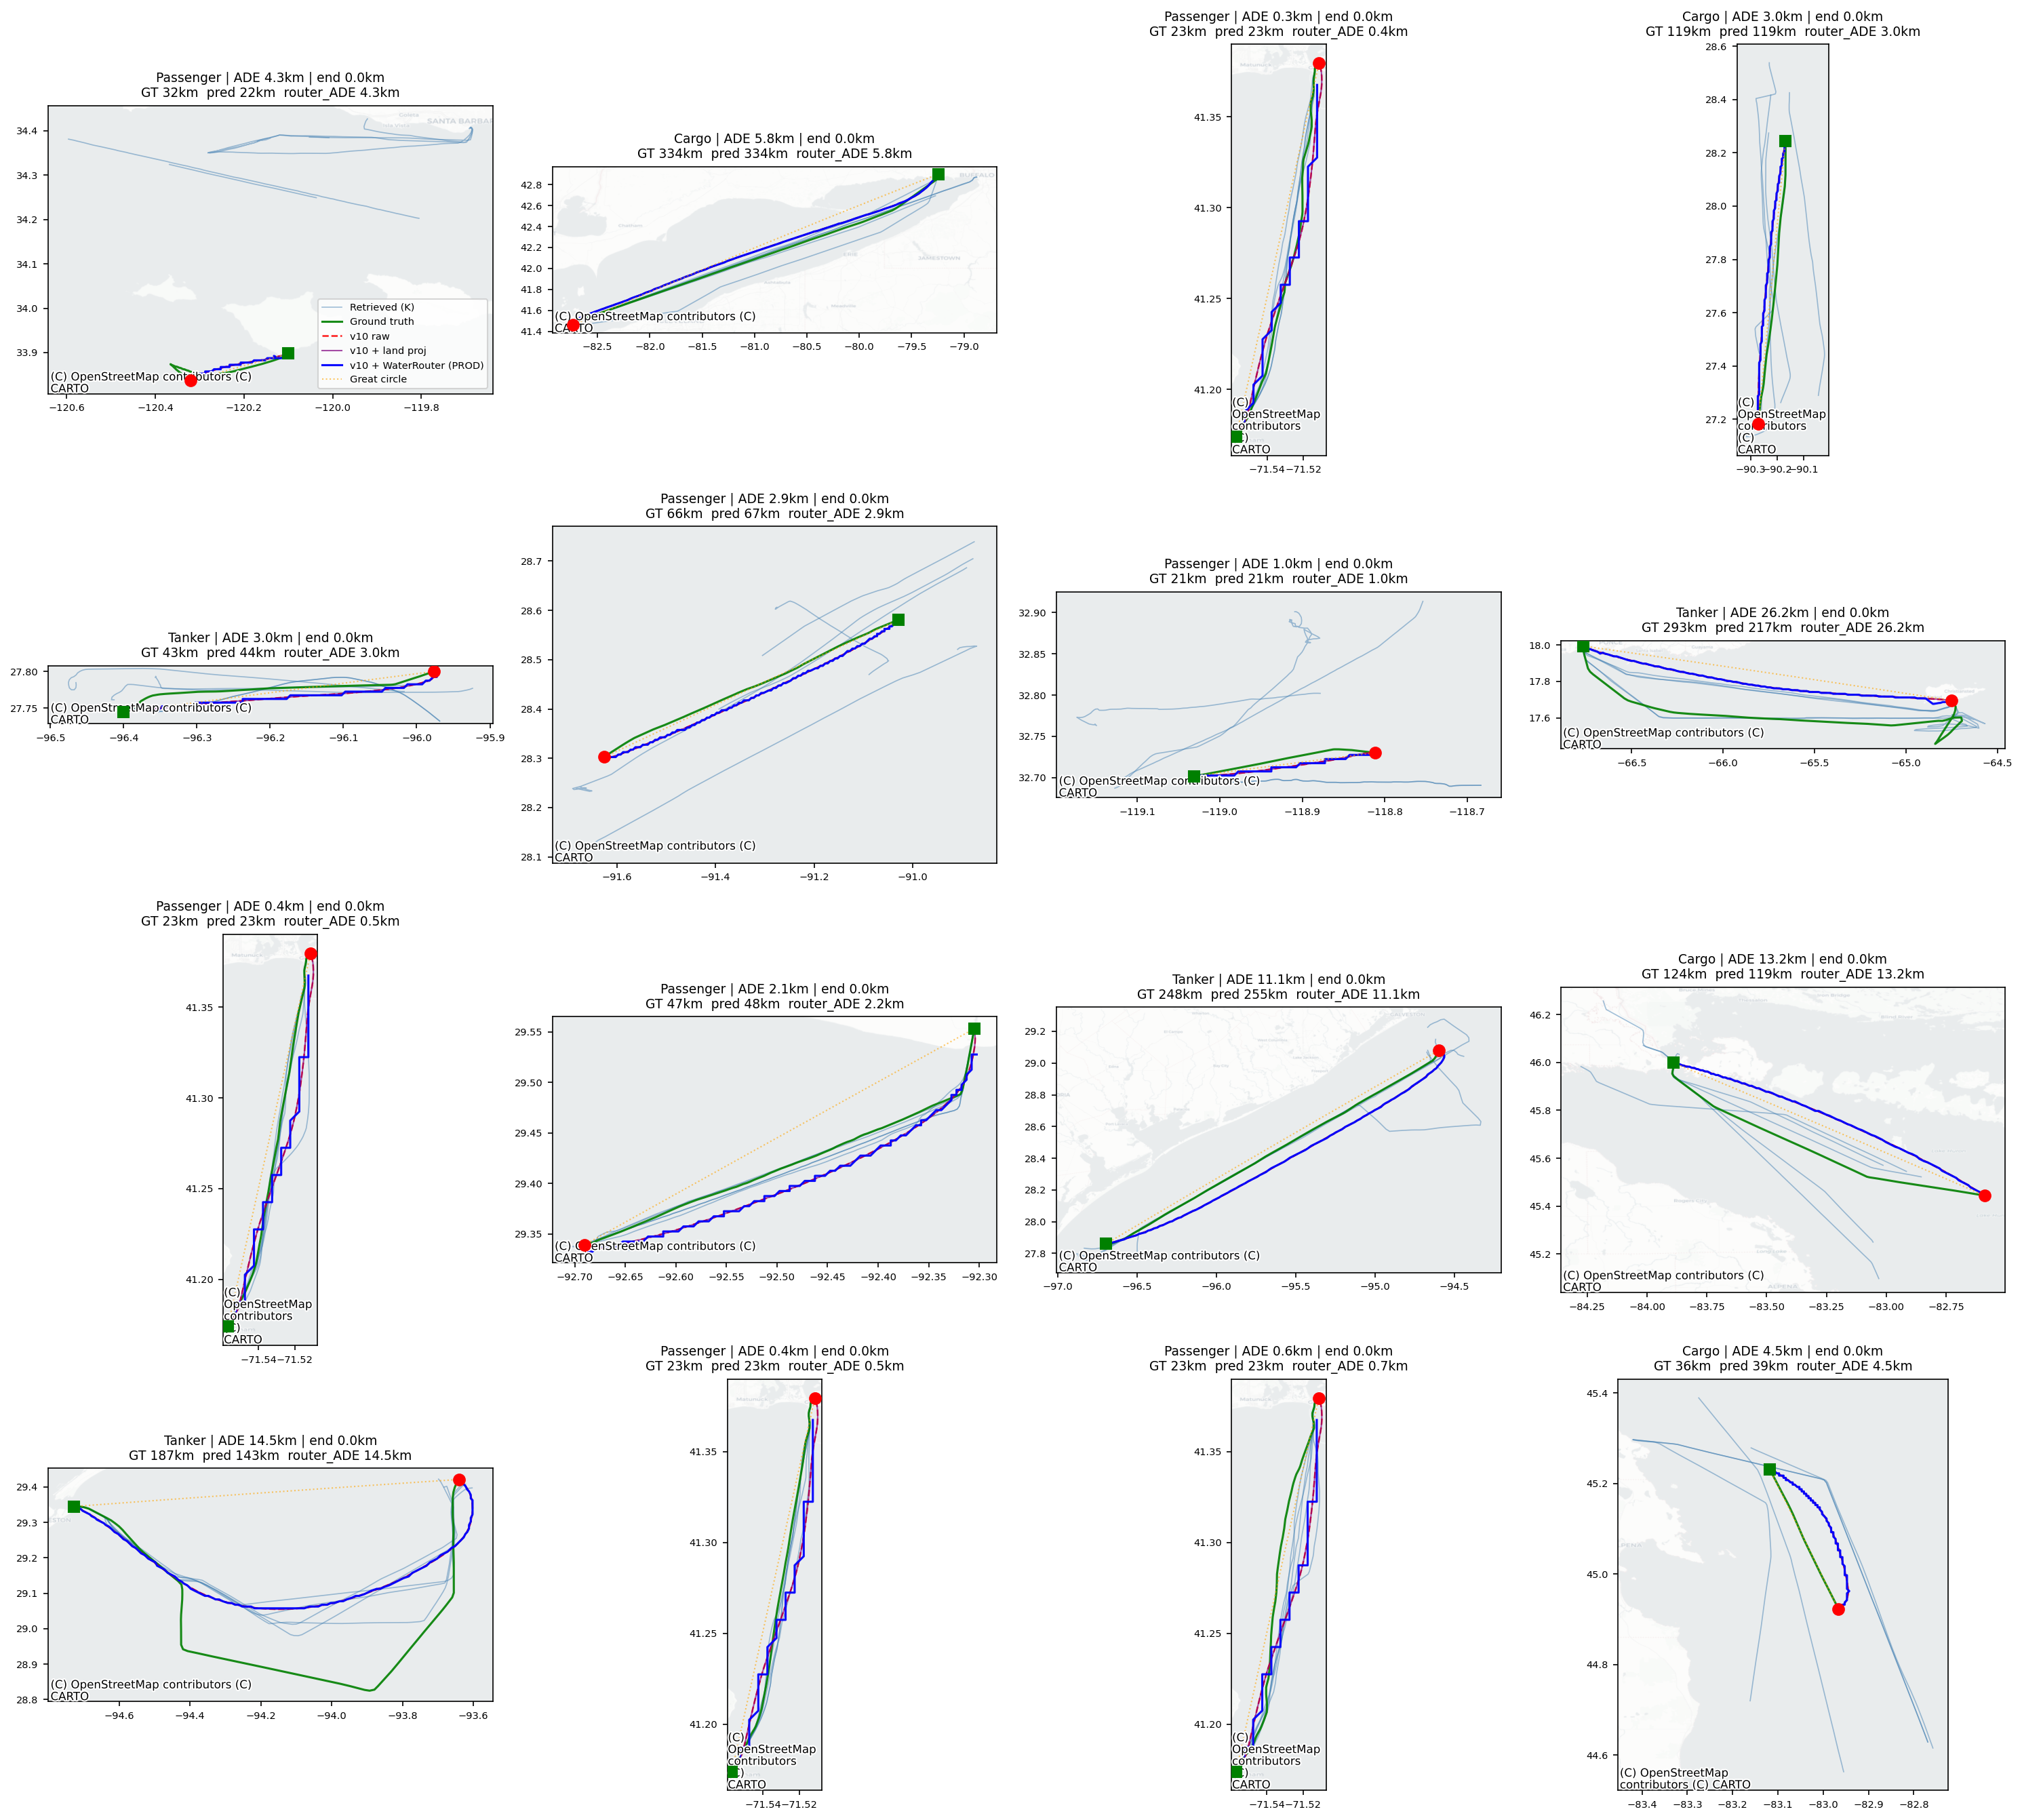
\includegraphics[width=\linewidth]{viz_v10_clean}
      \fcap{Generated routes (blue) vs ground truth}
  \end{columns}
  \vskip0.3em
  {\small\lead{Long ($>$500\,km):} 27.4\,km vs great-circle 60.1\,km - learned shipping-lane shape;
   \lead{short:} geodesic competitive.}
\end{frame}

% ---- 13. Robustness ------------------------------------------------
\begin{frame}{Robustness: stable across seeds}{The ranking and water-validity hold across 5 disjoint subsample seeds}
  \begin{columns}[c]
    \column{0.58\textwidth}\centering
      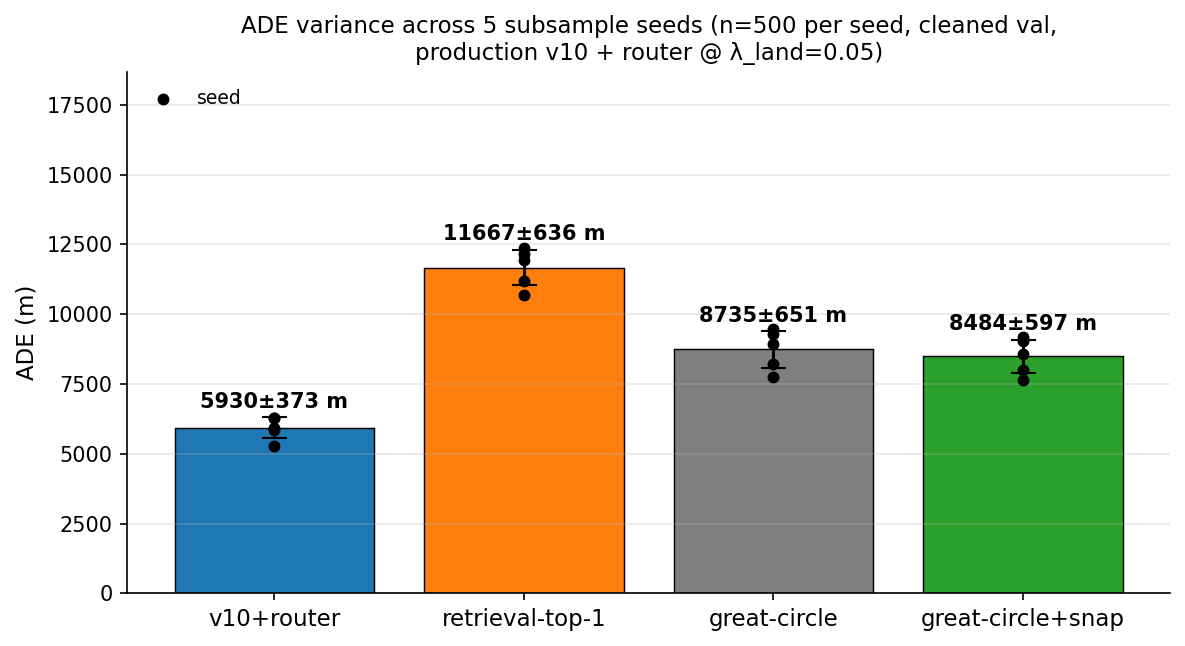
\includegraphics[width=\linewidth]{seed_variance}
      \fcap{ADE across 5 subsample seeds - v10+router vs baselines}
    \column{0.42\textwidth}
      \begin{itemize}\setlength\itemsep{0.8em}
        \item \lead{Tight spread:} production ADE $\pm225$--$372$\,m across seeds
        \item \lead{Ranking never flips:} v10+router lowest in every seed
        \item \lead{Always water-strict:} 0\% crossings in all 5 seeds
        \item \lead{Significant:} paired bootstrap CI vs great-circle excludes 0
      \end{itemize}
  \end{columns}
\end{frame}

% ---- 14. Lessons & conclusion --------------------------------------
\begin{frame}{Lessons, limitations \& outlook}
  \begin{itemize}\setlength\itemsep{0.3em}
    \item \lead{Retrieval = biggest architectural lever:} non-parametric memory beat 7 parametric ideas
    \item \lead{Data quality = biggest single intervention:} water-strict ADE $8898\to6051$\,m (same weights, dirty$\to$clean eval); crossings $\to$ 0
    \item \lead{Per-step loss $\neq$ rollout ADE:} only end-to-end evaluation should decide architecture
  \end{itemize}
  \vskip0.4em
  \begin{columns}[T]
    \column{0.5\textwidth}
      \begin{block}{Limitations}
        \small
        \begin{itemize}\setlength\itemsep{0.1em}
          \item Generator for \emph{known} waters - interpolates seen patterns
          \item Accuracy depends on retrieval-neighbour density
          \item No first-principles novel-geography reasoning
        \end{itemize}
      \end{block}
    \column{0.5\textwidth}
      \begin{block}{Outlook}
        \small
        \begin{itemize}\setlength\itemsep{0.1em}
          \item v13 - whole-sequence diffusion Transformer (EDM + CFG)
          \item Score-based land guidance during sampling
          \item Cross-region transfer \& multimodal sampling
        \end{itemize}
      \end{block}
  \end{columns}
\end{frame}

% ---- 15. Closing slide ---------------------------------------------
{\setbeamertemplate{footline}{}
\begin{frame}[plain]
  \begin{tikzpicture}[remember picture,overlay]
    \fill[epred] (current page.north west) rectangle ([yshift=-0.18cm]current page.north east);
    \fill[epred] ([yshift=0.18cm]current page.south west) rectangle (current page.south east);
  \end{tikzpicture}
  \vfill
  \begin{center}
    
\includegraphics[height=1.5cm]{logo-EP-vertical}\\[1.1em]
    {\Huge\bfseries\color{epnavy} Thank you}\\[0.6em]
    {\large\itshape\color{epgrey} Questions welcome}\\[1.1em]
    {\color{epred}\rule{3cm}{1.4pt}}\\[1.0em]
    {\normalsize\color{epnavy}\bfseries Andrei-Valentin \c{S}tirbu}\\[0.25em]
    {\small\color{epgrey} Generative Modelling of Maritime AIS Trajectories
     with Retrieval-Augmented Transformers}\\[0.2em]
    {\small\color{epgrey} Advisor: Davide Buscaldi - LIX, \'Ecole Polytechnique \& Sorbonne Universit\'e}
  \end{center}
  \vfill
\end{frame}}

\end{document}
